\chapter{Background}
\label{chap:background}

In this chapter I introduce the literature background for the thesis. I begin with a notation table used in the thesis and follow with a comprehensive overview of existing and examined SSL training frameworks, focusing on the architectures, training, evaluation, and downstream tasks. Then, I provide a breakdown on adversarial examples, with a focus on the main findings and universality, as well as the current attacks, and pair them with the current SSL paradigm.

\section{Notation}

The following table describes parts of the notation that is used throughout this work.

\begin{table}[h]
    \centering
    \small
    \resizebox{\textwidth}{!}{
        \begin{tabular}{ll}
        \toprule
        Symbol(s) & Meaning \\
        \midrule
        $c\in\{1, 2,...,K\}$; $K$ & Class; Number of possible classes \\
        $x\in\mathbb{R}^{C\times H\times W}$; $C$, $H$, $W$ & Image; Number of channels (usually 3), height, width. \\
        $z\in\mathbb{R}^d$; $d$ & Representation; Dimensionality of representation. \\
        $z^{(i)}$ & i-th element of the representation vector. \\
        $f_\theta: \mathbb{R}^{C\times H\times W}\rightarrow\mathbb{R}^d$; $\theta\in\Theta$ & SSL encoder; Parameters of the SSL encoder. \\ 
        $\mathcal{A}_i: \mathbb{R}^{C\times H\times W} \rightarrow \mathbb{R}^{C\times H\times W}$ & Image augmentation function (for example blurring). \\
        $\mathbb{A}=\{\mathcal{A}_1,\mathcal{A}_2,...\}$ & Set of augmentations. \\
        $D_T=\{(x_i,c_i)|i=1,...,N_T\}$; $N_T$ & A downstream training dataset; Number of samples. \\
        $l_\mathbf{w}: \mathbb{R}^d \rightarrow \mathbb{R}^K$;  $\mathbf{w}\in \mathbb{R}^{d\times K}$ & Linear downstream classification head; Parameters of $l_\mathbf{w}$. \\
        \bottomrule
        \end{tabular}
    }
    \label{tab:notation}
\end{table}

\section{SSL Image Encoders}\label{sec:ssl_bg}

I start by contrasting SSL with supervised learning task, like classification, which aims to predict a correct class $c$ from possible $K$ classes, based on the image $x$. Classifiers learn based on labeled data pairs $(x, c)$, under the supervised learning paradigm,~\ie the correct prediction is well known, and the sole training objective is to teach the NN to output a specific (correct) class $c$ for each image $x$.

SSL abandons the luxury of labeled data. Intuitively, most of the data one can obtain via Internet-scale scraping is unlabeled, and the labeling requires costly human labor. Without labels, SSL defines an alternative training objective,~\ie representation learning~\cite{ogssl}. Representations $z$ are understood as high-dimensional, continuous vectors. After training, the SSL model $f_\theta$ should output a rich and expressive representation $z$ of any image $x$, enabling further downstream use of the representations.

\subsection{Training Paradigms}\label{sec:ssl_training}

Notably, what exactly is a ``rich and expressive representation $z$ of any image $x$, enabling further downstream use of the representations'' is not well-grounded in theory, and does not have a clear formulation. Moreover, one cannot compute the gradient of such an objective to train a NN. 

A more precise view of the above goal is that: representations $z_1$, $z_2$ of two \textit{similar} images $x_1$, $x_2$ should be \textit{closer} than representations $z_1$, $z_3$ of two \textit{dissimilar} images $x_1$, $x_3$. Intuitively, an image of a dog should have a representation that lies close to other images of dogs in the embedding space and should have a representation that lies far away from images depicting circuit boards. 

\subsection{Similar Images and SSL}\label{sec:similar_imgs_ssl}

Defining ``similarity'' of images is tricky, especially since images can be similar in many ways. The similarity may be structural, compositional, semantic, stylistic, etc. To avoid ambiguities, and human-based biases, the default approach is to augment \textit{the same} image multiple times, producing multiple ``views'', since these views are (likely) similar to each other.

Representations' ``closeness'' is easier to precisely formulate. Since embeddings are continuous vectors, the natural approach is to use a \textit{similarity} function $\text{sim}: \mathbb{R}^d\times\mathbb{R}^d\rightarrow\mathbb{R}$, for example inverse L2 distance or cosine similarity. 

Effectively, given a dataset of $N$ unlabeled images $D=\{x_i|i=1,...,N\}$ the SSL training objective utilizing multiple views of the same image is as follows:

\begin{equation}
    \theta^*=\underset{\theta}{\argmax}
    \mathbb{E}_{x\sim D,\mathcal{A}_i\sim{\mathbb{A}},\mathcal{A}_j\sim\mathbb{A}}
        \left[\text{sim}\left(
            f_\theta\left(\mathcal{A}_i\left(x\right)\right),
            f_\theta\left(\mathcal{A}_j\left(x\right)\right)
        \right)\right]\text{.}
    \label{eq:loss_ssl_sim}
\end{equation}

\subsection{The Great Collapse}\label{sec:ssl_collapse}

Unfortunately,~\cref{eq:loss_ssl_sim} has a fatal flaw: its minimizer is a network $f_{\theta^*}: \mathbb{R}^{C\times H\times W}\rightarrow[0]^d$,~\ie always predicting a $d$-dimensional vector of zeros. 


\begin{wrapfigure}{r}{0.45\textwidth}
    \begin{center}
        \includegraphics[width=0.95\linewidth]{simsiam.pdf}
    \end{center}
    \caption{Visual depiction of the SimSiam framework, taken directly from~\cite{simsiam}.}
    \label{fig:simsiam}
\end{wrapfigure}

\paragraph{SimSiam}~\cite{simsiam} addresses this problem by \textit{stop-gradient operation}, and Siamese networks~\cite{siamese},~\ie two neural networks that share weights. During SimSiam training two views $x_1, x_2$ are passed through two encoders $f$ sharing the same weights, obtaining two representations $z_1, z_2$. Then, one of the representations (without loss of generality: $z_1$) is passed through an additional MLP prediction head $h$ to get $p_1=h(z_1)$. The training objective is to maximize $\text{sim}(p_1, z_2)$, with sim being cosine similarity. To avoid collapse, the gradients flowing \textbf{only} through the network (and $h$) that encoded $x_1$, while the update gradients based on $z_2$ are discarded, or in other words: stopped from flowing, hence the name \textit{stop-gradient}. This ensures that the network $f$ cannot ``cheat'' during training, to collapse to a trivial (and uninformative) solution of $[0]^d$ prediction regardless of the input image. Visual description of the SimSiam framework is shown in~\cref{fig:simsiam}.


\paragraph{DINO}~\cite{dinov1} presents another approach to solve the collapse problem. While still using the stop-gradient trick and dual-network stack, the encoders \textit{do not} share weights during training, at least not explicitly. Instead, they work in a student-teacher tandem, where the student encoder $f_S$ aims to match the representations of the teacher encoder $f_T$. Importantly, the views $x_S$ passed to the student are less informative than the views $x_T$ passed to teacher. The former are called \textit{local} views, and are of smaller resolution,~\ie obtained by more aggressive cropping, while the latter are \textit{global} views, covering over $50\%$ of the original image $x$. 

Unlike SimSiam, DINO's training loss is more involved. First, each dimension of the output representation is normalized using softmax function:
\begin{equation}
    \operatorname{softmax}(z^{(i)})=\frac{\exp(z^{(i)}/\tau)}{\sum_{k=1}^{d}\exp(z^{(k)}/\tau)}\text{,} 
    \label{eq:softmax}
\end{equation}
with $\tau>0$ being the temperature parameter, effectively turning it into probability distribution. Then, the training loss is based on cross-entropy loss:
\begin{equation}
    \text{CELoss}(y,\hat{y})=-y\log(y)\text{,} 
    \label{eq:celoss}   
\end{equation}
specifically, 

\begin{equation}
    \text{DINOLoss}=\text{CELoss}\left(\operatorname{softmax}\left(f_T\left(x_T\right)\right),\operatorname{softmax}\left(f_S\left(x_S\right)\right)\right)\text{.} 
\end{equation}
Stop-gradient operation is applied to the teacher network,~\ie the gradient update from the loss flows only through the student model. 

Note that the teacher model has to be updated too, for the student to be able to learn anything useful from it. The authors employ exponential moving average, with parameters of the teacher $\theta_T$ being updated using $\theta_T\leftarrow\lambda\theta_T+(1-\lambda)\theta_S$, with $\theta\in[0.996,1)$. Authors found it necessary to additionally \textit{center} the representations returned from the teacher, to encourage more uniform distribution of embeddings. To this end, they add a bias term $b$ to the output $f_T(x)\leftarrow f_T(x)+b$, with $b$ also being updated using exponential moving average after each batch: $b\leftarrow mb+(1-m)b\frac{1}{B}\sum_{i=1}^{B}f_T(x_i)$, where $B$ denotes the batch size, $x_i$---i-th element in the batch, and $m>0$ is the update rate parameter.

\subsection{Dissimilar Images and Contrastive Learning}

While \textit{similar} images' embeddings should stay close, prior work~\cite{simclr,clip} found it important that \textit{dissimilar} images' embeddings stay far away from each other. Analogously to~\cref{sec:similar_imgs_ssl}, it is not immediately clear what does exactly mean for two images to be dissimilar. 

The trivial solution is to assume that two different images are dissimilar (from the fact that they are \textit{different}), which is exactly what Contrastive Learning~\cite{contrastivelearningog} does. More precisely, instead of only matching two views of the same image, consider a batch of $B$ images, where each image has two distinct views, for a total of $2B$ views. Within $2B$ views, each view has exactly 1 positive view stemming from the same image, and $2B-1$ negative views, crafted from other images. Then, the InfoNCE~\cite{infonceloss} training loss on a pair of positive views $(x_i,x_j)$ is defined as:

\begin{equation}
    \label{eq:infonce}
    \text{InfoNCE}(x_i,x_j)=-\log\frac{
        \exp\left(\text{sim}\left(f\left(x_i\right),f\left(x_j\right)\right)/\tau\right)
        }{
        \sum_{k=1}^{2B}\mathbbm{1}_{[k\neq i]}\exp\left(
            \text{sim}\left(f\left(x_i\right),f\left(x_k\right)\right)/\tau
        \right)
    }
\end{equation}

Intuitively, this training objective forces the NN to ``push away'' the representations of all views of the alternative images from the positive views. Such a paradigm has been proven successful, with SimCLR~\cite{simclr} and CLIP~\cite{clip} achieving high quality representation expressiveness.

\subsection{Training Data}

Canonically~\cite{simclr,simsiam,dinov1}, pure-vision SSL encoders are trained for at most 100 epochs on an ImageNet-1k~\cite{imagenet} training set (1 million high-resolution images), to fix confounding variables when comparing different frameworks. However, since the SSL paradigm aims to enable training on \textit{any unlabeled data}, CLIP~\cite{clip} scaled training to 400 million samples collected from the Internet\footnote{CLIP uses image and text pairs for training, which is beyond the scope of this work.}, with \DINOvtwo~\cite{dinov2} following up with 142 million curated images for training, to maximize representation expressiveness.

\subsection{Encoder Architectures}

Since the SSL encoders considered in this work process images, the standard image processing NN architectures serve as the backbones for these models. ResNet~\cite{resnet}, an architecture which achieved state-of-the-art image classification capabilities before the dawn of Transformers~\cite{transformers}, is a popular choice,~\eg for SimSiam or SimCLR. The architecture is modified; instead of predicting a vector of per-class logit values, the final linear layer is removed, to expose features, which serve as representations. For more modern SSL encoders (CLIP, \DINOvone, \DINOvtwo), Vision Transformer~\cite{vit} (ViT) architecture is the default choice. ViT splits the image into a sequence of patches, and appends a \texttt{[CLS]} token to the sequence, representation of which canonically serves as an input to a classification layer (akin to the final ResNet linear layer). In the SSL setting, the representation of the \texttt{[CLS]} token is used as the image representation $z$.

\subsection{Evaluating SSL Image Encoders}\label{sec:eval_ssl}
The generality of the SSL training task (\cref{eq:loss_ssl_sim,eq:infonce}) comes at a cost. One can not simply look at the produced embeddings $z$ and assess their quality, since their dimension $d$ is often too high (above 100, sometimes even 1000) to allow for meaningful analysis, let alone a universal quality metric. Instead, researchers focus on measuring how useful the embeddings are to help solve well-defined tasks, like classification or semantic segmentation. 

\paragraph{Classification} is evaluated on a downstream dataset $D_T$ of $N_T$ labeled images. Based on the representations from trained $f_\theta$, a simple linear model $l_\mathbf{w}$ is fit, parameterized by $\mathbf{w}$, $l_\mathbf{w}(z)=\mathbf{w}^Tz$. Notably, only $\mathbf{w}$ is updated, and $\theta$ is kept frozen. Training minimizes cross-entropy loss~\cref{eq:celoss}. The final encoder+linear model classification stack is defined as $(l_\mathbf{w}\circ f_\theta): \mathbb{R}^{C\times H\times W} \rightarrow \mathbb{R}^K$, and its downstream task performance is evaluated as accuracy on the validation set of the training data $D_T$. 

\paragraph{Pixel-level} tasks, like semantic segmentation and depth estimation (evaluated in this work) require a more sophisticated approach. There, the dataset $D_T$ consists of images $x_i$ and ground-truth masks $m_i$. These tasks require two-dimensional, spatially aligned representations of the image to run predictions. Effectively, only ViT-based SSL encoders are applicable here, as they return a representation for each patch the input image is split into, contrary to a single 1D vector from ResNet. 

During inference, the image $x$ is split into $G=HW/P^2$ patches $\{\rho_i|i=1,...,G\}$,~\ie non-overlapping square crops of size $P\times P$ of the image $x$, and turned into a 1D sequence of patches, in a raster order (left to right, top to bottom). Encoder $f_\theta$ outputs a sequence of representations $\{z_i|i=1,...,G\}$ ($z_i\in\mathbb{R}^d$ is a representation of i-th patch $\rho_i$), which can be re-arranged back into a 2D grid of vectors, of size $(H/P)\times(W/P)$.

Prediction is akin to classification, where a linear model $l_\mathbf{w}$ is applied on representation of each patch separately, and scaled back to the original $H\times W$ size with linear interpolation.

\paragraph{Semantic segmentation} is a task to predict a class of \textit{each pixel}, with masks $m\in\{1,...,K\}^{H\times W}$, and the linear head $l_{\mathbf{w}}$ parameterized by $\mathbf{w}$. Training loss is cross-entropy loss (\cref{eq:celoss}) averaged over all pixels of the mask $\hat{m}$ predicted from image $x$, and its respective ground truth mask $m$:
\begin{equation}
    \text{SegCE}(m,\hat{m})=\frac{1}{HW}\sum_{i=1}^{H}\sum_{j=1}^{W}\text{CELoss}(m^{(i,j)},\hat{m}^{(i,j)})\text{.}
    \label{eq:seg_celoss}
\end{equation}

\paragraph{Depth estimation} task is to predict a continuous \textit{distance} of each pixel from the camera, where masks are $m\in\mathbb{R}_+^{H\times W}$. In this work, I follow the setup from \DINOvtwo~\cite{dinov2}, which is based on AdaBins~\cite{adabins}. 

Specifically, each per-patch representation $z_i$ is concatenated with the representation of the \texttt{[CLS]} token of the input image, effectively doubling the size of the input to the linear model $l_\mathbf{w}$ from $d$ to $2d$. To further increase the resolution of the predictions, the 2D grid of patch representations is upscaled by linear interpolation in each dimension, by a factor of $4$, effectively yielding $16\times G$ representation vectors.

Interestingly, in this setup the linear layer $l_\mathbf{w}$ \textit{does not directly predict} a continuous distance value for each patch, as might be suggested from the task description. Instead, the range of possible depths in the train dataset $\text{dep}\in[\text{dep}_\text{min},\text{dep}_\text{max}]$ is uniformly split into $256$ bins of identical width $b=(\text{dep}_\text{max}-\text{dep}_\text{min})/256$ (following \DINOvtwo~\cite{dinov2}). $l_\mathbf{w}$ outputs a probability distribution over the bins' centers, as if it was a classification or segmentation task, with $\mathbf{w}\in\mathbb{R}^{2d\times256}$. For representation $z_i$, the prediction is $p_i=\text{softmax}(l_\mathbf{w}(z_i))=\text{softmax}(\mathbf{w}^Tz_i)$, $p_i\in[0,1]^{256}$, assigning probability for each of the center $c_k=\text{dep}_\text{min}+\frac{2k-1}{2}b$, $k=1, 2, ..., 256$. The final prediction is a dot product between the vector of probabilities and vector of centers $\mathbf{c}=[c_1, c_2, ..., c_{256}]$,~\ie $\widetilde{\text{dep}_i}=\mathbf{c}^Tp_i$, and is computed for each representation $z_i$ for each patch $\rho_i$.

Similarly to semantic segmentation, per-patch predictions are concatenated, reshaped into a 2D grid, and rescaled to match the size of the input image $x$, using linear interpolation, obtaining prediction $\hat{m}$. The training loss for depth estimation is a weighted sum of two losses: \textit{multi-scale gradient matching} loss~\cite{depscaleloss} and \textit{pixel-wise depth loss}~\cite{adabins}. The former is computed over multiple scales $s\in\{(H/2^k,W/2^k)|k=0,1,2,3\}$, where the image at scale $s_k$ is downscaled to match the target size $(H/2^k,W/2^k)$, denoted $x_k$. The loss is:
\begin{equation}
    \text{DepScale}(m,\hat{m})=\frac{1}{HW}\sum_{k=0}^{3}
    \sum_{i=1}^{H/2^k}\sum_{j=1}^{W/2^k}\left(
        |\Delta_k^{(i,j+1)}-\Delta_k^{(i,j)}|+
        |\Delta_k^{(i+1,j)}-\Delta_k^{(i,j)}|
    \right)\text{,}
    \label{eq:depth_loss_scale}
\end{equation}
where $\Delta_k^{(i,j)}=\log\hat{m}_k^{(i,j)}-\log m_k^{(i,j)}$. This loss encourages more smooth predictions. Second term is 
\begin{equation}
    \text{DepPix}(m,\hat{m})=\alpha\sqrt{
        \frac{1}{HW}\sum_{i=1}^{H}\sum_{j=1}^{W}\left(\Delta^{(i,j)}\right)^2-
        \frac{\lambda}{H^2W^2}\left(\sum_{i=1}^{H}\sum_{j=1}^{W}\Delta^{(i,j)}\right)^2
    }\text{,}
    \label{eq:depth_pix}
\end{equation}
where $\alpha=1$, and $\lambda=0.85$, and explicitly penalizes the difference between ground truth and predicted depths. The final training loss is 
\begin{equation}
    \text{DepLoss}(m,\hat{m})=0.5\text{DepScale}(m,\hat{m})+\text{DepPix}(m,\hat{m})\text{.}
    \label{eq:deploss}
\end{equation}


\section{Adversarial Examples}\label{sec:advex_bg}

While most of the field focused on making the models better and more general,~\cite{advex} identified a grave vulnerability of almost every neural network that exists. With some assumptions and little effort, \textbf{any NN} can be forced to output a wrong prediction with high consistency. What is even worse, such an adversarial input to the NN can be made almost indistinguishable from a real, benign input, and can evade detection. Changing a few pixel values by tiny values (for example by at most 8/255 of the full pixel range) is enough to reliably fool a vast majority of image-based NNs, regardless of their training data, training objective, architecture, hyperparameters, preprocessing, and so on.

\begin{figure}[t]
    \vspace{-.05in}
    \small
    \centering
\begin{tabular}{
    >{\centering\arraybackslash}m{.2\textwidth}
    >{\centering\arraybackslash}m{.1\textwidth}
    >{\centering\arraybackslash}m{.225\textwidth}
    >{\centering\arraybackslash}m{.075\textwidth}
    >{\centering\arraybackslash}m{.225\textwidth}
    }
    \centering\arraybackslash
%abs max for panda was 138, eps was 1., so relative eps is ~.007
    
\includegraphics[width=.2\textwidth]{panda_577.png} &%
    $\ +\ .007\ \times$ &%
    
\includegraphics[width=.2\textwidth]{nematode_082.png} &%
    $=$ & %
    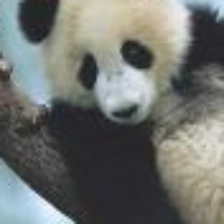
\includegraphics[width=.2\textwidth]{gibbon_993.png} \\
    ``panda'' &                & ``nematode''     &   & ``gibbon'' \\
    57.7\% confidence &        &   8.2\% confidence & & 99.3 \% confidence
\end{tabular}
\caption{Example of adversarial example that fools an image classifier. Left: original image $x$. Middle: adversarial perturbation $\sign(\nabla_x\text{CELoss}(f_V(x),y))$. Right: adversarial image $x+\epsilon\sign(\nabla_x\text{CELoss}(f_V(x),y))$, with $\epsilon=0.007$. Sourced from the seminal work on adversarial examples~\cite{fgsm}.}
\label{fig:fgsm}
\end{figure}

Authors of~\cite{advex} dubbed their discovery as ``adversarial examples''. More precisely, an adversarial example $x_{adv}$ is an image close to a benign image $x$, crafted explicitly to cause misprediction of a victim model $f_V$. To limit the difference between clean and adversarial image, $\left\|x_{adv}-x\right\|$ is oftentimes constrained to be within an $\epsilon$-ball,~\ie $\left\|x_{adv}-x\right\|_p<\epsilon$, where $p\in\{0,1,2,\infty\}$. To ensure imperceptibility, $\epsilon$ is usually very small,~\eg $8/255$ for $L_\infty$ norm~\cite{pgd,carliniandwagner}, meaning each pixel of the image is changed by at most $8/255$ (assuming pixel values are in $[0,1]$).

Another important element of adversarial examples is the optimization procedure to obtain $x_{adv}$. To cause a misprediction in the classification setting, one can maximize the CELoss, eventually flipping the predicted label from correct to incorrect. Specifically, given image $x$ and its label $y$, FGSM~\cite{fgsm} computes 
\begin{equation}
    x_{adv}\leftarrow x+\epsilon\sign(\nabla_x\text{CELoss}(f_V(x),y))\text{.}
    \label{eq:fgsm}
\end{equation}
The added perturbation consists only of $\{-\epsilon,\epsilon\}$ values, where the sign is determined to maximize the CELoss between the prediction of $f_V$ on $x$ and the ground truth label $y$. One of the well-known examples of FGSM is presented in~\cref{fig:fgsm}, with an image classifier being forced to mispredict an obvious image of panda after very small amount of noise added. Note that the perturbation $\sign(\nabla_x\text{CELoss}(f_V(x),y))$ is obtained \textit{in a single forward and backward pass}, making this attack both very effective, and very cheap to execute.

While single-step FGSM already achieves impressive results, one can do better by using an iterative approach. Specifically, projected gradient descent \PGD~\cite{pgd} performs $T$ update steps of~\cref{eq:fgsm} to further strengthen the attack. Full attack can be found in~\cref{alg:pgd}.

\begin{algorithm}
\caption{PGD~\cite{pgd} algorithm.}
\label{alg:pgd}
\begin{algorithmic}
    \Require $\epsilon$ (maximum perturbation strength), $\eta$ (step size), $T$ (total iterations)
    \Require Obj (optimization objective,~\eg CELoss), clip, $(x,y)$, $f_V$
    \Ensure $x_{adv}$, s.t. $\|x_{adv}-x\|_\infty\leq\epsilon$, and $f_V(x_{adv})\neq y$ (if attack succeeds)
    \State $\delta\sim\mathcal{U}[-\epsilon, \epsilon]^{C\times H\times W}$ \Comment{Sample the initial perturbation}
    \State $x_{adv}\gets x+\delta$ \Comment{Initialize $x_{adv}$}
    \For{step $t=1,...,T$}
        \State $x_{adv}\gets x_{adv}+\eta\sign\left(\nabla_x\text{Obj}\left(f_V\left(x\right),y\right)|_{x=x_{adv}}\right)$ \Comment{See~\cref{eq:fgsm}}
        \State $x_{adv}\gets x+\text{clip}(x_{adv}-x,-\epsilon,\epsilon)$ \Comment{Ensures $\left\|x_{adv}-x\right\|_\infty\leq\epsilon$}
    \EndFor
\end{algorithmic}
\end{algorithm}

While \PGD and FGSM perform very well against simple classification tasks, more complex problems like semantic segmentation require a more involved approach. \SegPGD~\cite{segpgd} identifies that a na\"{\i}ve application of \PGD attack to the segmentation loss (averaged CELoss on each pixel) does not necessarily maximize the \textit{absolute number} of mis-predicted pixels within the image $x_{adv}$. Instead, they split the predicted pixels $\hat{m}$ into two groups: correctly classified ($\hat{m}_+$), and incorrectly classified ($\hat{m}_-$). The goal of \SegPGD is to maximize the size of the latter set. The optimization objective of \SegPGD is a weighted sum of losses on both sets:
\begin{equation}
    \begin{aligned}
        \text{SegPGD}(f_V,x_{adv},m,,t)=\frac{1-\lambda(t)}{HW}\sum_{(i,j)\in \hat{m}_+}CELoss(f_V(x_{adv})^{(i,j)},m^{(i,j)})+\\
        \frac{\lambda(t)}{HW}\sum_{(k,l)\in \hat{m}_-}CELoss(f_V(x_{adv})^{(k,l)},m^{(k,l)})\text{,}
    \end{aligned}
    \label{eq:segpgd}
\end{equation}
with $\lambda(t)=(t-1)/2T$ being the weighting factor, step-dependent. The objective function~\cref{eq:segpgd} can be easily plugged into the \PGD algorithm (\cref{alg:pgd}), in place of Obj.
